\documentclass[
    a4paper, % Stock and paper size.
    9pt, % Type size.
    % article,
    % oneside, 
    onecolumn, % Only one column of text on a page.
    % openright, % Each chapter will start on a recto page.
    % openleft, % Each chapter will start on a verso page.
    openany, % A chapter may start on either a recto or verso page.
    ]{memoir}
\usepackage[utf8]{inputenc}
\usepackage[T1]{fontenc}
\usepackage{lmodern}
\usepackage[final]{microtype}
\usepackage[dvips]{graphicx}
\usepackage{xcolor}
\usepackage{tikz}
\usepackage{caption}
%\usepackage{times}

% Comment in final version
\usepackage{todonotes}
\usepackage{soul}

%\usepackage[margincaption,outercaption,ragged,wide]{sidecap}
\usepackage[margincaption,ragged]{sidecap}
\sidecaptionvpos{figure}{t} 
\sidecaptionvpos{table}{t}

\usepackage[
breaklinks=true,colorlinks=true,
%linkcolor=blue,urlcolor=blue,citecolor=blue,% PDF VIEW
linkcolor=black,urlcolor=black,citecolor=black,% PRINT
bookmarks=true,bookmarksopenlevel=2]{hyperref}

\usepackage{geometry}
% PDF VIEW
% \geometry{total={210mm,297mm},
% left=25mm,right=25mm,%
% bindingoffset=0mm, top=25mm,bottom=25mm}
% PRINT
% \geometry{total={210mm,297mm},left=20mm,right=50mm,bindingoffset=10mm, top=25mm,bottom=25mm}

% Code from https://tex.stackexchange.com/questions/275565/tufte-layout-in-painless-memoir

% Start code

% MEMOIR LAYOUT
\setlength{\baselineskip}{14pt}
\setlength{\normalbaselineskip}{14pt}

% GEOMETRY
\settrims{0pt}{0pt}
\settypeblocksize{49\baselineskip}{107mm}{*}
\setlrmargins{24.8mm}{*}{*}
\setulmargins{27.4mm}{*}{*}
\setheadfoot{\baselineskip}{\baselineskip}
\setheaderspaces{*}{2\baselineskip}{*}
\setmarginnotes{8.2mm}{49.4mm}{\onelineskip}
\checkandfixthelayout


% TEXT
% ragged2e provides ragged justification with hyphenation
\RequirePackage{ragged2e}
\AtBeginDocument{\RaggedRight}
\setmpjustification{\RaggedLeft}{\RaggedRight}
\setlength{\RaggedRightParindent}{1.0pc}
\setlength{\parindent}{1pc}
\setlength{\parskip}{0pt}
% linespacing ~ 14pt
\linespread{1.17}

% text styling of all side footnotes
\renewcommand{\footnotesize}{\fontsize{8pt}{10pt}\selectfont}
\renewcommand{\foottextfont}{\footnotesize}
% styling and placement of mark
\footmarkstyle{{#1. }}
\setlength{\footmarkwidth}{0em}
\setlength{\footmarksep}{-\footmarkwidth}
% memoir command - do all footnotes in margin
\footnotesinmargin


% SIDECAPTIONS
\setsidecaps{\marginparsep}{\marginparwidth}
\sidecapmargin{outer}
\setsidecappos{t}
\renewcommand*{\sidecapstyle}{%
\captionnamefont{\foottextfont\scshape}
\ifscapmargleft
\captionstyle{\RaggedLeft\footnotesize\foottextfont}%
\else
\captionstyle{\RaggedRight\footnotesize\foottextfont}%
\fi}

% FULLWIDTH environment
% The following code should be used *after* any changes to the margins and
% page layout are made (e.g., after the geometry package has been loaded).
\newlength{\fullwidthlen}
\setlength{\fullwidthlen}{\marginparwidth}
\addtolength{\fullwidthlen}{\marginparsep}

% \newlength{\fullwidthlen}
% \setlength{\fullwidthlen}{\marginparwidth}
% \addtolength{\fullwidthlen}{\marginparsep}

\newenvironment{fullwidth}{%
  \begin{adjustwidth*}{}{-\fullwidthlen}%
}{%
  \end{adjustwidth*}%
}


% End code

%

\OnehalfSpacing
%\linespread{1.3}

% disable by disabling the todo notes
\makeatletter
 \if@todonotes@disabled
 \newcommand{\hlnote}[2]{#1}
 \else
 \newcommand{\hlnote}[2]{\todo{#2}\texthl{#1}}
 \fi
 \makeatother

%%% CHAPTER'S STYLE
%\chapterstyle{bianchi}
%\chapterstyle{ger}
\chapterstyle{dash}
%\chapterstyle{madsen}
%\chapterstyle{ell}
%%% STYLE OF SECTIONS, SUBSECTIONS, AND SUBSUBSECTIONS
\setsecheadstyle{\Large\bfseries\sffamily\raggedright}
\setsubsecheadstyle{\large\bfseries\sffamily\raggedright}
\setsubsubsecheadstyle{\bfseries\sffamily\raggedright}


%%% STYLE OF PAGES NUMBERING
\pagestyle{companion}\nouppercaseheads 
\pagestyle{headings}
\pagestyle{Ruled}
%\pagestyle{plain}
\makepagestyle{plain}
\makeevenfoot{plain}{\thepage}{}{}
\makeoddfoot{plain}{}{}{\thepage}
\makeevenhead{plain}{}{}{}
\makeoddhead{plain}{}{}{}

%%% For parts with abstracts on the page

\usepackage{xpatch}

\makeatletter
\xpatchcmd{\part}{\null\vfil}{\vspace*{.1\textheight}}{}{}

\providecommand{\abstractname}{Content of this part}
\newenvironment{partwithabstract}
  {\begingroup\let\@endpart\relax\part@withabstract}
  {\endquotation\endgroup\@endpart}
\newcommand{\part@withabstract}{\@dblarg\part@@withabstract}
\def\part@@withabstract[#1]#2{%
  \part[#1]{#2}%
  \vfil
  \begin{center}\bfseries\abstractname\vspace{-.5em}\vspace{\z@}\end{center}
  \quotation
}
\makeatother




\maxsecnumdepth{subsection} % chapters, sections, and subsections are numbered
\maxtocdepth{subsection} % chapters, sections, and subsections are in the Table of Contents

\usepackage[backend=biber]{biblatex}
\addbibresource{library.bib}

%% make a glossary
\usepackage[acronym, xindy, nonumberlist]{glossaries}
\makeglossaries


\newglossaryentry{weaklysupervisedl}
{
        name={Weakly Supervised},
        description={Weakly supervised machine learning where the ground truth labels are only partially available. 
        In the context of image segmentation, this can mean that the labels are only provided at image level or that point level annotation in the image is provided.
        The model is trained on incomplete labels, the desired result remains the complete segmentation of the image.
        Just like in the case of \textit{Fully Supervised Learning} the objective is to model the relationship between an \textit{input} and an \textit{output}. 
        Due to the labels being incomplete, there is a stronger need to identify the internal structure of the data, as is the case for \textit{Unsupervised learning}.
        }
}

\newglossaryentry{segmentation}{
        name={Segmentation},
        description={
                The \textit{segmentation} problem in machine vision consists of the classification of each individual pixel or voxel. 
                The problem of \textit{semantic} segmentation is to detect, for each pixel, the object category it belongs to. 
                \textit{Instance} segmentation digs deeper. It identifies for each pixel the object instance it belongs to.
                The difference is that it differentiates between two objects of the same object category in the picture. 
                }
        }

\newglossaryentry{groundtruth}{
        name={Ground Truth},
        description={
                The \textit{Ground Truth} is a term used in machine learning to indicate the ideal expected result. 
                In the context of Instance Segmentation, the ground truth is the true class of every pixel or voxel. 
        }
        }

\newglossaryentry{unsupervisedl}
{
        name={Unsupervised},
        description={
                In an \textit{Unsupervised} machine learning problem, no labels are present. 
                The aim is not to model the relationship between an \textit{input} and an \textit{output}, the aim is to model the structure of the data.
                \todo[inline]{Add examples of algorithms? KNN, MoG}
                }
}

\newglossaryentry{supervisedl}
{
        name={Supervised},
        description={
                (Fully) Supervised Machine Learning task where target labels are present. 
                The objective of these problems is to model the relationship between an \textit{input} and an \textit{output}.
                \todo[inline]{Add examples of algorithms?}
                }
}

\newglossaryentry{tomography}
{
        name={Tomography},
        description={
                Imaging of a volume through the use of a penetrating wave. 
                Through these waves, a collection of images, called \textit{tomograms}, are produced.
                The mathematical procedure to reconstruct the original volume based on these images is called \textit{tomographic reconstruction}.
                A \acrfull{ct} scan is produced through tomographic reconstruction of several X-ray radiographs.
                }
}

\newglossaryentry{machinevision}
{
        name={Machine vision},
        description={
                The branch of Artificial Intelligence with the objective of invering results from images. 
                In this work, these images can be both two dimensional (\textit{pictures}) as three dimensional (\textit{volumes}).
                }
}

\newglossaryentry{ai}
{
        name={Artificial Intelligence},
        description={
                The study of using computers to automatically perform tasks which once were considered only humans could do.
                This includes, but is not restricted to, interpretation of speech and images. It is often refered to with the acronym \textsc{ai}.
                }
}

\newglossaryentry{deepl}
{
        name={Deep Learning},
        description={
                Deep learning is a branch of Machine Learning where a set of multiple sequential layers is used to progressively extract higher-level features from the raw input data.
                }
}

\newglossaryentry{caml}
{
        name={Class Activation Maps},
        description={
                Technique to identify region of an image \textit{responsible} for the classification result.
                }
}


\newacronym{cnn}{CNN}{Convolutional Neural Network}
\newacronym{crf}{CRF}{Conditional Random Field}
\newacronym{ct}{CT}{Computer Tomography}
\newacronym{mri}{MRI}{Magnetic Resonance Imaging}
\newacronym{ml}{ML}{Machine Learning}
\newacronym{mil}{MIL}{Multi-Instance Learning}
\newacronym{rnn}{RNN}{Recurrent Neural Network}
\newacronym{us}{US}{Ultra Sound imaging}


%%%---%%%---%%%---%%%---%%%---%%%---%%%---%%%---%%%---%%%---%%%---%%%---%%%

\begin{document}

\newgeometry{total={210mm,297mm},left=30mm,right=30mm,bindingoffset=5mm, top=25mm,bottom=25mm} 

%%%---%%%---%%%---%%%---%%%---%%%---%%%---%%%---%%%---%%%---%%%---%%%---%%%
%   TITLEPAGE
%
%   due to variety of titlepage schemes it is probably better to make titlepage manually
%
%%%---%%%---%%%---%%%---%%%---%%%---%%%---%%%---%%%---%%%---%%%---%%%---%%%
\thispagestyle{empty}

{%%%
\sffamily
\centering
\Large

~\vspace{\fill}

{\huge 
Spine vertebrae segmentation in 3D CT scan images
}

\vspace{2.5cm}

{\LARGE
Jan Alexander
}

\vspace{3.5cm}

A thesis submitted in partial fulfillment for the\\
degree of Master in Statistical Data Analysis\\[1em]
in the\\[1em]
Faculty of Science\\
Universiteit Gent

\vspace{3.5cm}

Supervisors:\\
Dr. Joris Roels\\
Dr. Bert Vankeirsbilck

\vspace{\fill}

September 2021

%%%
}%%%

\cleardoublepage
%%%---%%%---%%%---%%%---%%%---%%%---%%%---%%%---%%%---%%%---%%%---%%%---%%%
%%%---%%%---%%%---%%%---%%%---%%%---%%%---%%%---%%%---%%%---%%%---%%%---%%%

\tableofcontents*

\clearpage

%%%---%%%---%%%---%%%---%%%---%%%---%%%---%%%---%%%---%%%---%%%---%%%---%%%
%%%---%%%---%%%---%%%---%%%---%%%---%%%---%%%---%%%---%%%---%%%---%%%---%%%

\glsaddall
\setglossarystyle{listdotted}
\printglossary[type=\acronymtype]
\glossarystyle{altlist}
\printglossary

\clearpage

%\cleardoublepage
\restoregeometry
\chapter*{Abstract}
\addcontentsline{toc}{chapter}{Abstract}

% Set page layout to plain (only page number) and two-column 
\begin{multicols}{2}
\thispagestyle{plain}
\par{
    \textit{
        Medical professionals use \acrfull{mri} or \acrfull{ct} scans as essential components for medical diagnosis, following the course of medical conditions and the planning of medical procedures.
        There is a trend towards machine vision to support medical professionals interpreting and using these images.
        Building these applications requires expensive labelled datasets.
        This research investigates techniques to reduce the dataset labelling cost by working with point annotation instead of full annotation.
        Experiments are conducted on publicly available datasets and demonstrate two new loss components and a combination technique of different model results to generate pseudo masks.
        As a final result, this work demonstrates that one can obtain 72 \% of the performance of a fully annotated model at an estimated 24 \% of the labelling cost. 
    }
}
\section*{Thesis objective \& Motivation}
\par{
    The use of radiological images is a crucial element in modern medical practice. 
    \acrshort{mri} or \acrshort{ct} scans are essential components for pre-operative and post-operative diagnosis, following the course of medical conditions and the planning of medical procedures.
    Automated interpretation of medical images can mean a gain in efficiency.
}
\par{
    Machine vision - deep learning in general - tends to be very \textit{data-hungry}. Constructing a new model requires large, labelled datasets.
    Acquiring these datasets and the corresponding labels is time-consuming and expensive. 
    Maximisation of the return of a given data and labelling budget through is a goal shared by all \acrshort{ml} practitioners.
    The use of weak labels, or sometimes called \textit{hints}, is one approach to attempt this.
    This approach aims to train a model capable of inferring more informative results than the information level explicitly available in the labelling.
}
\par{
    This project presents a model for the automated segmentation of the lumbar vertebrae of the human spine based on point level annotated medical scans.
    Point level annotation is faster and cheaper than providing a complete label mask (estimated at 8.4\% of cost\cite{Bearman2015}), this technique provides a cost-benefit. 
    The labels only contain the true class of a mere handful of voxels. This is a weak label to classify all voxels.
}



\section*{Data sets and data preprocessing \label{sec:abstr_data}}
\par{
    All datasets used in this work are publicly available (all datasets are listed on page \pageref{sec:datasets}). 
    These datasets contain both \acrshort{ct} and \acrshort{mri} scans. 
    In 86 of these scans, complete volume masks of the vertebrae are available. 
    In 20 volumes, only semantic labels are available.
    For 125 volumes, point level annotation is available.
}
\par{
    The complete dataset of 231 patients consists of 112 women and 99 men. Of 23 people, no gender information is available. 
    Since a medical professional does not order a medical scan unless there is a suspicion of a medical condition, the dataset contains various patients with different pathologies,
    such as patients with scoliosis and with crushed and wedged vertebrae.
}
\par{
    Different datasets vary in data formats and different scan resolutions. 
    Data preprocessing starts with homogenising the scan resolution by resampling the image on an $1mm\times 1mm\times 1mm$ grid. 
    Next, the image is sliced along one of the three principal axes.
    The contrast of the 2D image slices is first enhanced with the \acrfull{clahe} algorithm.
    Then the images are cropped (or padded, if needed) to form $352 px \times 352 px$ slices.
    All models are built with this image size, sufficient to contain all 5 lumbar vertebrae $L_1$ to $L_5$ in one image.
}


\section*{Methodology}
\par{
    The performances of different models are compared based on the class-weighted dice score.
    This metric takes into account both the model precision and recall as well as the class imbalance.
}
\par{
    For 86 scans, full annotation masks are available.
    As a performance benchmark, the performance of a fully supervised model trained on these images ($Dice_w=0,76$) is taken.
}
\subsection*{Weakly supervised models}
\par{
    The model backbond is the VGG16-FCN8 network, pre-trained on a large classification dataset.
    The model estimates 6 segmentation classes (5 lumbar vertebrae and the background class). 
    By training three different weakly supervised models on sets of 2D images sliced along the 3 main volume dimensions, three sets of segmentation masks are obtained. 
    The combination of these different segmentation masks is used as an \textit{pseudo} label set to train a fully supervised model on one volumetric dimension.
}

\subsubsection*{Loss function}
\par{
    To train the weakly supervised network, several loss components, both supervised and unsupervised, are combined.
    The model loss to train three point-supervised models in the first step of the procedure presented in this work consistents of 4 components:
    the point loss $\mathcal{L}_P$ and the consistency loss $\mathcal{L}_C$ were defined in \cite{Laradji2021} by I. Laradji, while this work introduced the prior extend and separation loss components $\mathcal{L}_E$ and $\mathcal{L}_S$ are introduced in this work.
}
\par{
    The weighted cross-entropy loss is optimised for the fully supervised reference model, a classic choice for this problem.
    It is also the point loss $\mathcal{L}_P$ component of the weakly supervised model. Then it is only evaluated on the set of available point labels $\mathcal{I}_i$.
    The function combines the six network output channels with a softmax function $\sigma$, after which the negative log-loss function is calculated, weighted with factors $w$.
}
\begin{equation} \label{eq:crossEntropy}
    \mathcal{L}_P(X_i) = -\sum_{\vec{p} \in \mathcal{I}_i} w_{\mathcal{Y}_i(\vec{p})}.\log\left[\sigma_{\mathcal{Y}_i(\vec{p})}\left(\vec{z_i(\vec{p})}\right)\right]
\end{equation}
\par{
    The unsupervised rotation consistency loss $\mathcal{L}_C$ imposes that the model output $f_\theta$ should be consistent for a transformation $t_k$ of the input image.
    In this work, the chosen transformations are image rotations over $0^\circ, 90^\circ, 180^\circ$ or $270^\circ$, combined with an image flip.
}
\begin{equation}
    \mathcal{L}_C(X_i) = \sum_{p \in \mathcal{P}_i} \left| t_k\left[f_\theta(X_i)\right]_p - f_\theta\left( t_k[X_i] \right)_p  \right|  
\end{equation}
\par{
    The second unsupervised loss term is the separation loss term. 
    Due to the low volume of labelled voxels, the the model lacks the incentive to output differentiating expressions of the output channels $\vec{z}_i$.
    $\mathcal{L}_S$ forces the model to do this.
}
\begin{equation}
    \mathcal{L}_S(X_i) = - \sum_{\vec{p}} \sum_{m\in \mathcal{K}} \sum_{n \in \mathcal{K}, n>m} \mathbf{S}(z_i[m]) - \mathbf{S}(z_i[n])
\end{equation}
\par{
    Finally, $\mathcal{L}_E$, the maximal extend supervised loss term, takes into account that a lumbar vertebra has a limited size ($r=110mm$).
    The Euclidian distance field $\mathbf{d}$ from the annotation point is converted to a semi-mask for each class $k$:
    \begin{eqnarray}
        \mathbf{d}_k(\vec{q}) &=& \max_{\vec{p}:\mathcal{Y}_i(\vec{p})=k}||\vec{q} - \vec{p}||\\
        \mathbf{m}_k(\vec{q}) &=& \mathbf{I}\left( (-\mathbf{d}(\vec{q}) + r) > 0 \right)
    \end{eqnarray}
    Now, $\mathbf{m}$ is 1 only for positions closer than distance $r$ from the annotation points for class $k$.
    Where $\mathbf{m}_k=0$, the model output should not indicate output class $k$. Where $\mathbf{m}_k=1$, the output class is unknown.
    The loss function is the binary cross-entropy between $\mathbf{m}_k$ and the sigmoid of the k$^{th}$ channel of the logits $z_i$ with weight vector $\{1, 0\}$.
}
\begin{equation}
    \mathcal{L}_E(X_i) = \sum_{k\in\mathcal{K}}\sum_{\vec{q}\in X_i}  (1-\mathbf{m}_k(\vec{q})) \log(\mathbf{S}(z_i(\vec{q})_k)) 
\end{equation}

\subsubsection*{Model result combination}
\par{
    Combining the results of the three models trained on the three geometric axes (transverse, frontal \& sagittal) is a pseudo-mask of higher quality than the results of the individual models.
    After morphological smoothing, the pseudo mask is used to train the final model (on sagittal slices).
}
\thispagestyle{plain}
\section*{Results}
\subsection*{Hyperparameter optimization}


\subsection*{Final result}

\section*{Conclusion}
\todo[inline]{Complete this section}
\cleardoublepage
\end{multicols}
\newgeometry{total={210mm,297mm},left=20mm,right=20mm,bindingoffset=5mm, top=25mm,bottom=25mm} 
\begin{partwithabstract}{Problem Introduction \& Motivation}
    The objective of this project is the development of a model for the automated vertebrae instance segmentation of \acrshort{mri} and \acrshort{ct} scans of the lumbar part of the human spine based on point annotated training data.
    
    This part of the book aims to clarify these terms. 
    I start off with some information regarding the human spine and the medical imaging techniques to investigate it.
    Secondly, I define and clarify different machine learning problems and techniques when working with two and three dimensional images.
    This part of the book ends with a discussion of previous work. 
    First the previous work to tackle the problem of instance segmentation of the human spine from medical images.
    Then prevous work in the field of \Gls{weaklysupervisedl} \Gls{machinevision}.
\end{partwithabstract}

\restoregeometry
\chapter{The human spine}\thispagestyle{empty}
\par{
    This document presents a model for automatic segmentation of \acrfull{ct} and \acrfull{mri} images of the lumbar spine.
    This chapter introduces these terms\footnote{This work is not a medical desideration. For in-depth knowledge on the anatomy and physiology of the spine, consult the specialized literature.}.
    Secondly, it gives a basic overview of the medical imaging techniques. 
    Finally, it touches upon a specific medical procedure in which this information is used: the minimally invasive surgery of a spinal hernia.
}
\section{Anatomy of the human spine}

\par{
    The spinal column, vertebral column or backbone\footnote{NL: \textit{wervelkolom}} is a structure of 34 bones. 
    It holds the body upright while providing it with the mobility to bend and twist.
    the \textit{intervertebral discs} make this possible. These consist of a ring of fibrocartilage and an inner gel-like centre and form an articulation between two vertebrae.
    Moreover, the vertebral column serves as a conduit for significant nerves running from the brain to the toes.
    The spinal column, as illustrated in figure \ref{fig:spineimage} can be divided into five regions:
}
\begin{description}
    \item[the Cervical spine:] 7 vertebrae of the neck, indicated by $C1$ to $C7$\footnote{Vertebrae are numbered from the head down. C1 (\textit{atlas}) is the vertebra closest to the head}.
    \item[the Thoracic spine:] 12 vertebrae of the middle back ($T1$ to $T12$).
    \item[the Lumbar spine:] 5 vertebrae that form the lower back. These are commonly referenced as $L1$ to $L5$.
    \item[the Sacrum:]\footnote{NL: \textit{Heiligbeen}} This is a structure consisting of 5 naturally fused vertebrae ($S1$-$S5$).
    \item[the Coccyx:]\footnote{NL: \textit{Stuit of staartbeen}} Structure of 3 to 5 naturally fused vertebrae at the end of the spinal column.
\end{description}


\begin{SCfigure}[][h!]
    \centering
    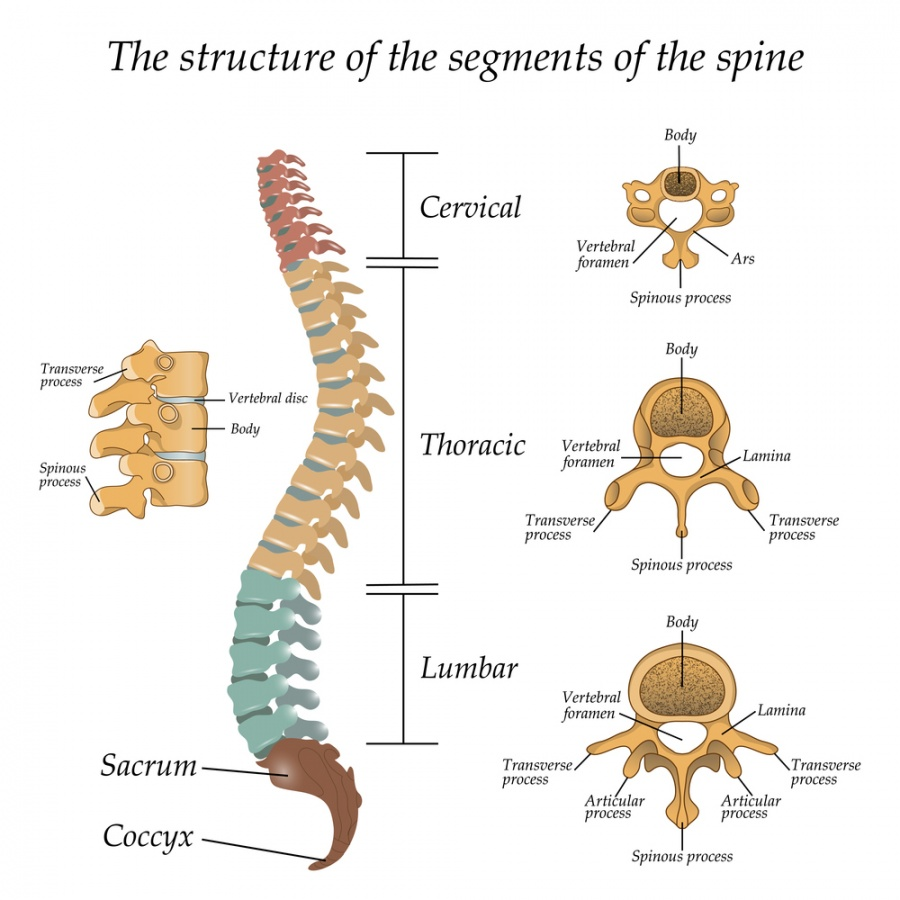
\includegraphics[width=10cm]{/home/thesis/images/SpineModel.jpeg}
    \caption{\label{fig:spineimage}Model of the human spine. The five vertebrae in green form the lumbar spine. They are referred to as \textit{L1} to \textit{L5} from top to bottom. Image source: \url{shutterstock.com}}
\end{SCfigure}

\section{Pathologies of the human spine}
\par{
    This document does not aim to provide an exhaustive list of all human spinal pathologies. 
    Two pathologies are interesting to discuss further as an introduction to this work since they occur in the data used in this project (see page \pageref{sec:datasets} for further details).
}
\begin{SCfigure}[][h!]
    \centering
    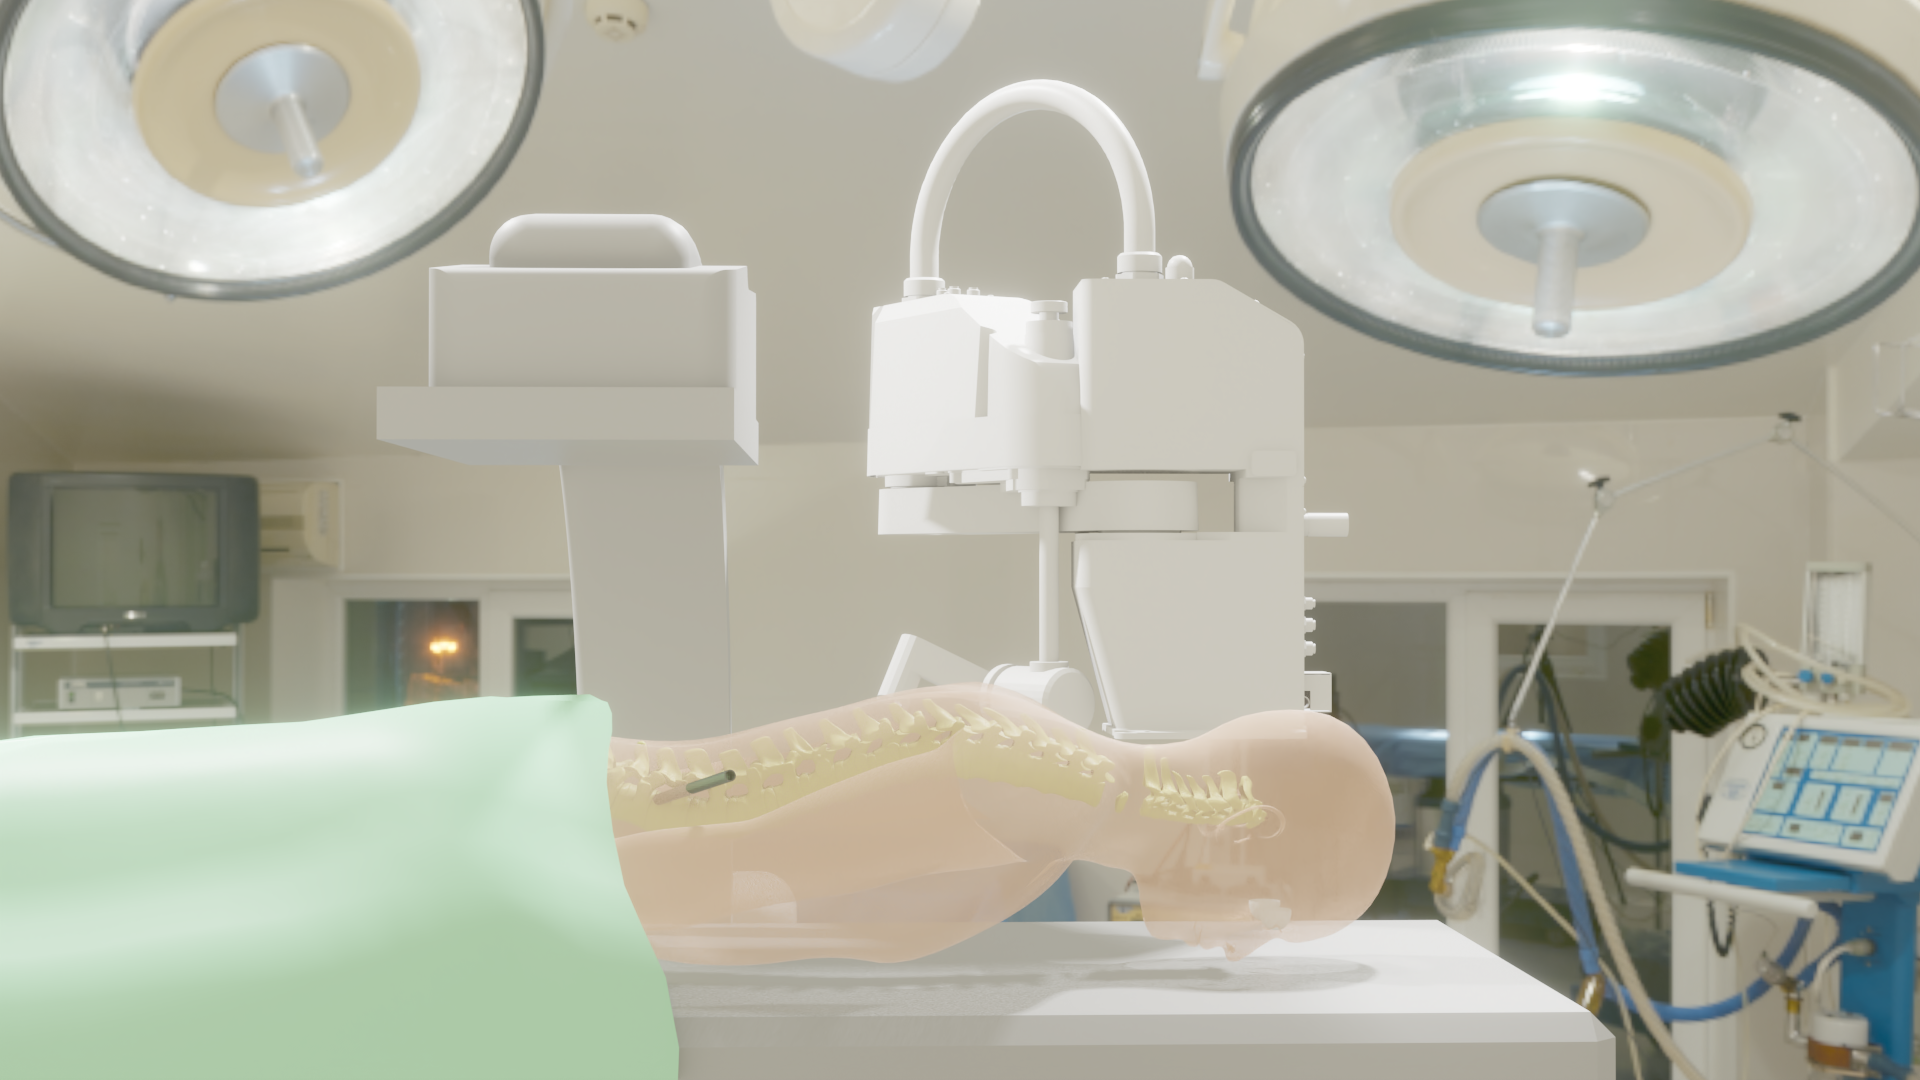
\includegraphics[width=10cm]{/home/thesis/images/REISS_illustration.png}
    \caption{Artist's impression of the start of the surgical treatment of a lumbar hernia. 
    This image shows the dilator through which the surgical instruments will be inserted to mill away the bulging disc material.
    This procedure requires repeated visualization of the instruments and the spine via X-ray images. \textit{This illustration is designed by Verhaert NP\&S}.\label{fig:REISS_procedure}}
\end{SCfigure}
\par{
    First, there is \textit{scoliosis}, which is a sideways curve of the spine.
    The severity of this condition can vary from relatively mild to severe. 
    In severe cases, scoliosis can affect the patient's movement and breathing.
}
\par{
    Second, there is the \textit{spinal hernia} or spinal disc herniation\footnote{Spinal disc herniation is sometimes referred to as a \textit{slipped disc}.}. 
    A spinal hernia is caused by damage to the \textit{annulus fibrosus}\footnote{The fibrocartilage ring around the softer gel-like centre of the intervertebral disc.}. 
    This damage can cause the intervertebral disc to bulge out. 
    This condition is painful due to the inflammation reaction, and in severe cases, the bulging material can irritate or cause impingement of the critical nerves along the spine.
    The nerve impingement can even lead to radiating pain to the limbs or even limb paralysis.
    In severe cases, a spinal hernia requires surgical treatment.
    This specialized procedure requires repeated medical imaging to allow the surgeon to accurately investigate the situation before the operation and assure correct positioning of the instruments during the intervention.
}
\par{
    In image \ref{fig:REISS_procedure}, the start of the surgical treatment procedure for a lumbar hernia is illustrated.
    One possible benefit of improved automatic interpretation of \acrshort{mri} and \acrshort{ct} scans is providing support for this procedure.
    This delicate procedure requires interpreting and registering information from both scan types (at different times), a demanding task for which automated support could be helpful.
    Image registration of the pre-operative \acrshort{mri} scan with the operation planning to the imaging of the situation on the operation table starts by segmentation of the affected vertebrae.
}

\section{Medical imaging of the human spine\label{sec:medical_imaging}}
\marginpar{
        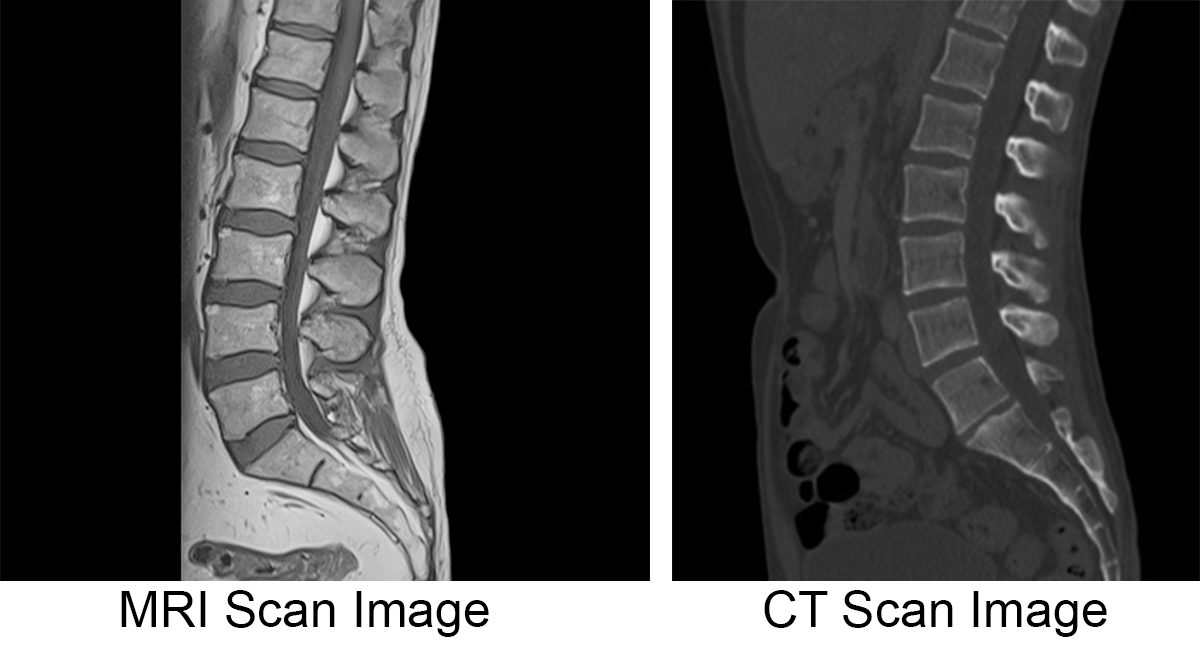
\includegraphics[width=5cm]{/home/thesis/images/MRI_CT_images.jpeg}
        \captionof{figure}{Illustration of \acrshort{ct} and \acrshort{mri} images of a human lumbar spine.}
        \label{fig:mri_ct}
    }
\par{
    For diagnosis and visualization of spinal pathology several medical imaging techniques are used: \acrfull{ct}, \acrfull{us} and \acrfull{mri}. 
    These techniques allow non-invasive visualization of the spine and discs in three dimensions.
    Slices from volumetric scans (\acrshort{mri} and \acrshort{ct}) are illustrated in \ref{fig:mri_ct}.
}

\subsection{CT scan}
\par{
    The \acrfull{ct}\footnote{Also known as CAT-scan, for Computed Axial Tomography or Computer-assisted Tomography.} is a non-invasive medical imaging procedure
    \footnote{\Gls{tomography} scans are primarily used for medical purposes. 
    It is also used in the industry for non-destructive inspection of components and assemblies.
    In geology, it is used to identify materials in a drill core quickly. In archaeology, it is used for the non-destructive investigation of artefacts. } 
    for diagnostic purposes. 
    A \acrlong{ct} procedure consists of the combination of an array of X-ray attenuation images taken with a rotating X-ray tube as illustrated in figure \ref{fig:CT_principle}. 
    These images can be combined with a \Gls{tomography} algorithm to reconstruct a volumetric representation of the radiographic density.
}
\par{
    Contrary to \acrfull{mri} imaging, this technique is suitable for patients with a pacemaker or insulin pump since there are no magnetic fields involved.
    The main disadvantage of \acrshort{ct} is the exposure to ionizing radiation\footnote{Radiation exposure increases the probability of cancer.} of the patient and the risk of exposure of the medical professional to the same radiation.
    The image quality increases with radiation dose, but so does the radiation exposure.
    Improving the reconstruction algorithms to obtain higher-resolution images while reducing radiation is an ongoing area of research. 
}
\marginpar{
        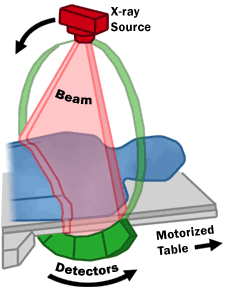
\includegraphics[width=5cm]{images/FDA_CT_Scan.png}
        \captionof{figure}{Conceptual illustration of the working of a \acrlong{ct} scan. Image from \url{www.fda.gov/radiation-emitting-products/medical-x-ray-imaging/computed-tomography-ct}}
        \label{fig:CT_principle}
    }

\subsection{MRI scan}
\par{
    The \acrfull{mri} scan is a medical imaging technique that is not based on ionizing radiation\footnote{Eventhough the alternative name \textit{nuclear} magnetic resonance (NMR) might confuse.}.
    \acrshort{mri} imaging will visualize the concentration of hydrogen\footnote{In theory, other atoms than hydrogen can be excited by adapting the excitation frequency.} atoms.
    The patient is positioned in a tunnel where a high constant magnetic field is applied. 
    A temporary oscillating signal is applied with the resonance frequency corresponding to hydrogen atoms is superposed on the static magnetic field.
    The hydrogen atoms will fall back to the equilibrium state, emitting radiofrequency (RF) signals, measured by receiving coils.
    \acrlong{mri} is particularly suitable for visualization of tissue with higher water content, such as tumours and infections, and to visualize fat.
}
\par{
    An \acrshort{mri} scan can be \textit{T1 weighted} or \textit{T2 weighted}. 
    A T1 weighted image is constructed based on the relaxation time of the magnetization is colinear with the direction of the static field
    while T2 weighted images are based on the magnetization perpendicular to the static field.
    While areas with higher water content, such as infected areas, will release a higher signal on a T2-weighted \acrshort{mri} scan, the same images will show a lower signal strength for T1-weighted scans.
}
\par{
    Contrary to \acrfull{ct} scans, the \acrlong{mri} procedure does not expose the patient of radiation. 
    Due to the high magnetic fields, the technology cannot be used for patients with pacemakers, cochlear implants or other metallic objects in the body.
    \acrshort{mri} allows to visualize soft tissue better than \acrshort{ct} images. An \acrshort{mri} image allows visualizing both the grey and white brain matter, while this is not possible with \acrshort{ct} images.
    Although both techniques produce images that resemble each other, none can replace the other one completely.
}


\chapter{Machine vision}

\Gls{machinevision} is the branch of \Gls{ai} focussed on image processing.
The machine vision task performed in this work is called instance \Gls{segmentation}.
In this chapter, I explain what this means. 
The task of segmentation is compared to other machine vision tasks.

This work investigates the used of \Gls{weaklysupervisedl} data for training an Instance segmentation model. 
The concept and benefits of \Gls{weaklysupervisedl} machine learning are explained.

\section{Machine vision tasks \label{sec:machinevisiontasks}}

\Gls{machinevision} is a broad discipline. 
Humans extract information from images almost subconsciously and we are often not aware of the different tasks we perform on images.
The objective of this section is to briefly define different machine vision tasks discussed further in this book. 
Several machine vision tasks consist of \textit{recognizing} objects, animals or humans in an image.
A model is build for a finite list of \textit{categories} that can be present in an image.
Depending on the question asked ad inference time, on can distinquish the following tasks.

\begin{description}
    \item[Image classification] is the task of determining what object category\footnote{or categories} is present in the image. Is there a cat in this image?
    \item[Object counting] is the task of counting how many instances of each category can be seen in the image. How many cats are there in this picture? 
    \item[Object detection] consists not only of identification of the object. Also the spatial position is requested. This is often requested in the form of a bounding box. Where is the cat in this picture, if a cat is present?
    \item[Semantic segmentation] requires that for each image pixel, a class is estimated. Pixels that do not belong to a specific class are called the \textit{background}.
    \item[Instance segmentation] requires not only that the semantic class is determined for each pixel, but also that two individuals of the same class\footnote{say, two cats.} are distinguished.   
\end{description}

The difference between these machine vision tasks is illustrated in figure \ref{fig:machinevisiontasks}. 

\begin{SCfigure}[][h!]
    \centering
    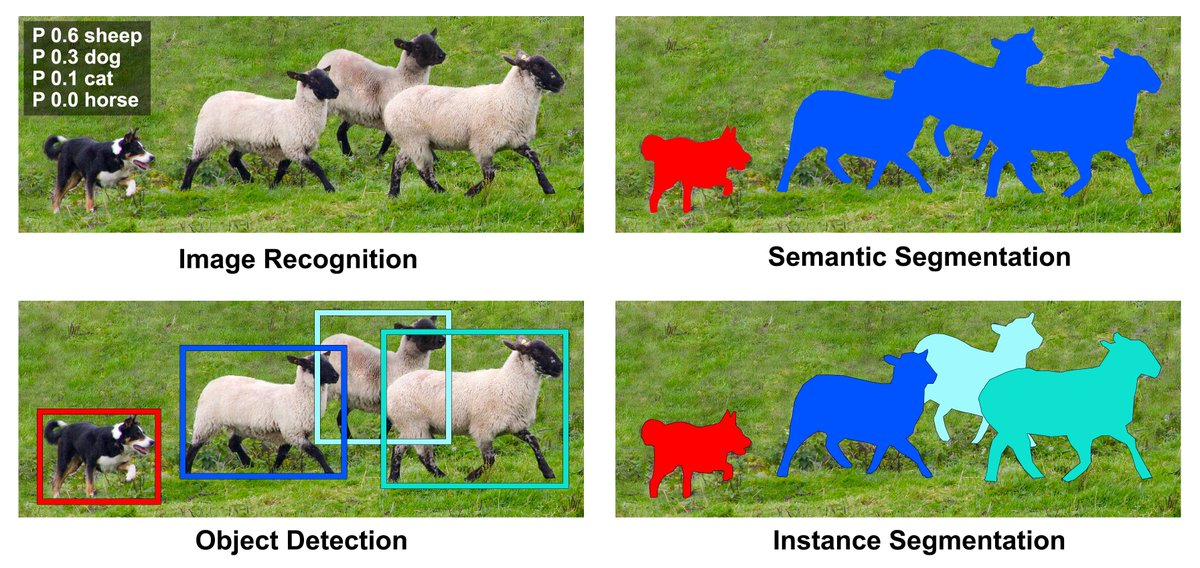
\includegraphics[width=10cm]{/home/thesis/images/Classification_vs_Segmentation.jpg}
    \caption{Illustration to compare different Machine vision tasks \cite{SemTorch76:online}. 
    Object detection means that the location of several objects is estimated by the model. This is indicated by the \textit{bounding boxes}.
    Segmentation of an image is the process of classifying each pixel in the correct class or assign it to the \textit{background} class.
    Semantic segmentation makes no difference between different instances of the same semantic class, instance segmentation does.
    \label{fig:machinevisiontasks}}
\end{SCfigure}

Other interesting applications of \gls{machinevision} include\footnote{This list is not exhaustive.}:
\begin{description}
    \item[Face recognition] is the identification of human faces. 
    \item[Image reconstruction] or \textit{inpainting} consists of recreating parts of a damaged image.
    \item[Image captioning] consists of the creation of full sentences describing the content of an image.    
\end{description}



\section{Supervision types}

To build a model to perform the tasks discussed in \ref{sec:machinevisiontasks}, this model needs to be trained.
This requires a set of \textit{labelled} images. 
This means that a collection of images needs to be provided where an expert in the intended task has provided correct information the model can \textit{learn} from.
Depending on the model objective, other types of labelling are required.
Figure \ref{fig:ImageLabelTypes} illustrates several types of image supervision : 
Point supervision, squiggle, bounding box and full mask.
The generation of these labels is very expensive and time-consuming.
Especially \gls{deepl} models are known to be very data-hungry. 
These models have determined unprecedented performance, provided sufficient data has been provided.

\begin{SCfigure}[][htb]
    \centering
    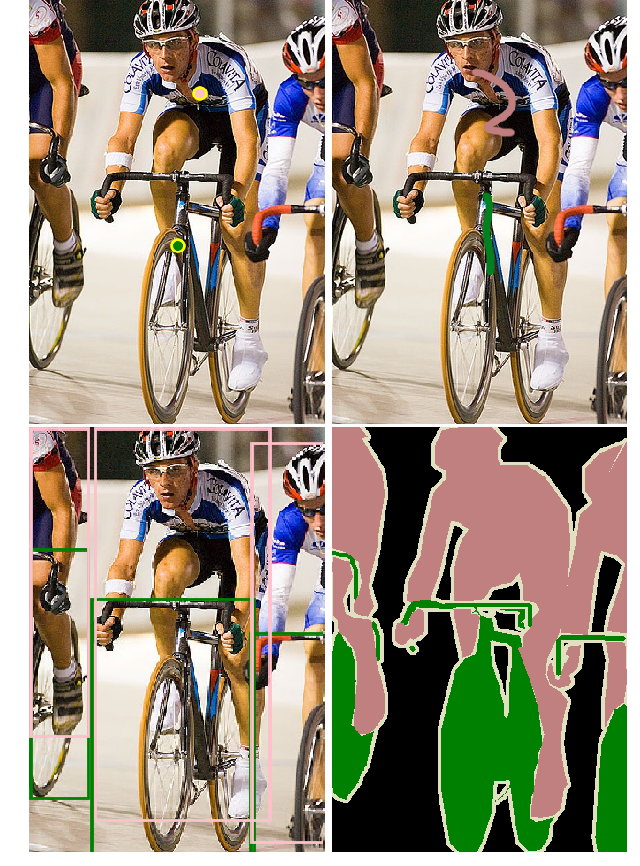
\includegraphics[width=10cm]{/home/thesis/images/McEver.png}
    \caption{Four different annotation types \cite{McEver2020}: 
    On the top left the picture is point level annotated. The points are inflated for visibility.
    On the top right, squiggle annotation is used.
    The bottom left shows bounding box supervion.
    While the bottom right image is fully annotated.
    An image level label would indicate that there are multiple instances of \textit{person} and \textit{bike} in the image.
    \label{fig:ImageLabelTypes}}
\end{SCfigure}

Given the high labelling cost, several researchers have investigated ways to train computer vision models with cheaper labels.
This branch of research is known as \Gls{weaklysupervisedl}.
The objective is to construct a strong model based on \textit{cheap} (incomplete, noisy or imprecise) labels. 
This is sometimes described as \textit{indirect supervision}.
Numerous creative approaches have been conceived. 
It is impossible to give an exhaustive list of approaches. 
In what follows, I will mainly focus on the approaches I chose to investigate myself, but I will also try to give some hints of the remarkable creativity found in the field.
Since the provided annotations in \Gls{weaklysupervisedl} are not full labels, these are sometimes described as \textit{hints} instead\footnote{
    This is based on the insightfull talk at \url{
        https://youtu.be/4EjYxVVCAaE
    }. For example, the destinction between labels and hints.
}.
The basic concept of \Gls{weaklysupervisedl} is that there are two sources of information to draw from: The hints and the prior knowledge about the problem (Priors).
These \textit{Priors} can be any form of prior knowledge about the object to be segmented\footnote{or any other machine vision task.}.
Priors can be the object size, shape or location, the number of instances, the similarity across images or the similarity with exernal images.

Wether an annotation is considered a \textit{weak label} or a \textit{strong label} depends more on the modellers intend than on the annotation itself. 
Basically, when one aims to construct a model to infer output labels with a higher informative value than the original annotations, these \textit{labels} become \textit{hints}.
Making a model to predict bounding boxes from a dataset annotated with bounding boxes means considering these as \textit{strong labels}. 
If one uses the same dataset to construct a model that predicts pixel-wise masks, you use the labels as \textit{weak labels} or \textit{hints}.

For a segmentation task, weak labels can be:
\begin{description}
    \item[Image level labels]: When only  
\end{description}

\todo[inline]{Motivation of weakly supervised learning --> Difference in annotation time and cost from Bearman and Laradji Covid}
\chapter{Previous work}

This project sits at the intersection of two areas of research. 
First there is the application of \Gls{ai} in medical applications, specifically for segmentation problems.
Then, there is the active area of research of \Gls{weaklysupervisedl} machine learning.

\section{Artificial intelligence for medical applications}

\todo[inline]{Start with short overview of other AI problems (~5 lines)}

\Gls{ai} has proven to be a valuable contribution to medical practice to reduce the burden of repetitive tasks on the medical caregiver.

\todo[inline]{elaborate: ppg to blood pressure - slaapapnue}

\section{Segmentation problems for medical applications}

\todo[inline]{General introduction of U-Net and other medical approaches}

For segmentation tasks, the U-net \cite{Ronneberger2015} is widely used. 
This architecture can be represented by a characteristic U-shape, as the name indicates.
It consists of 

\begin{SCfigure}[][htb]
    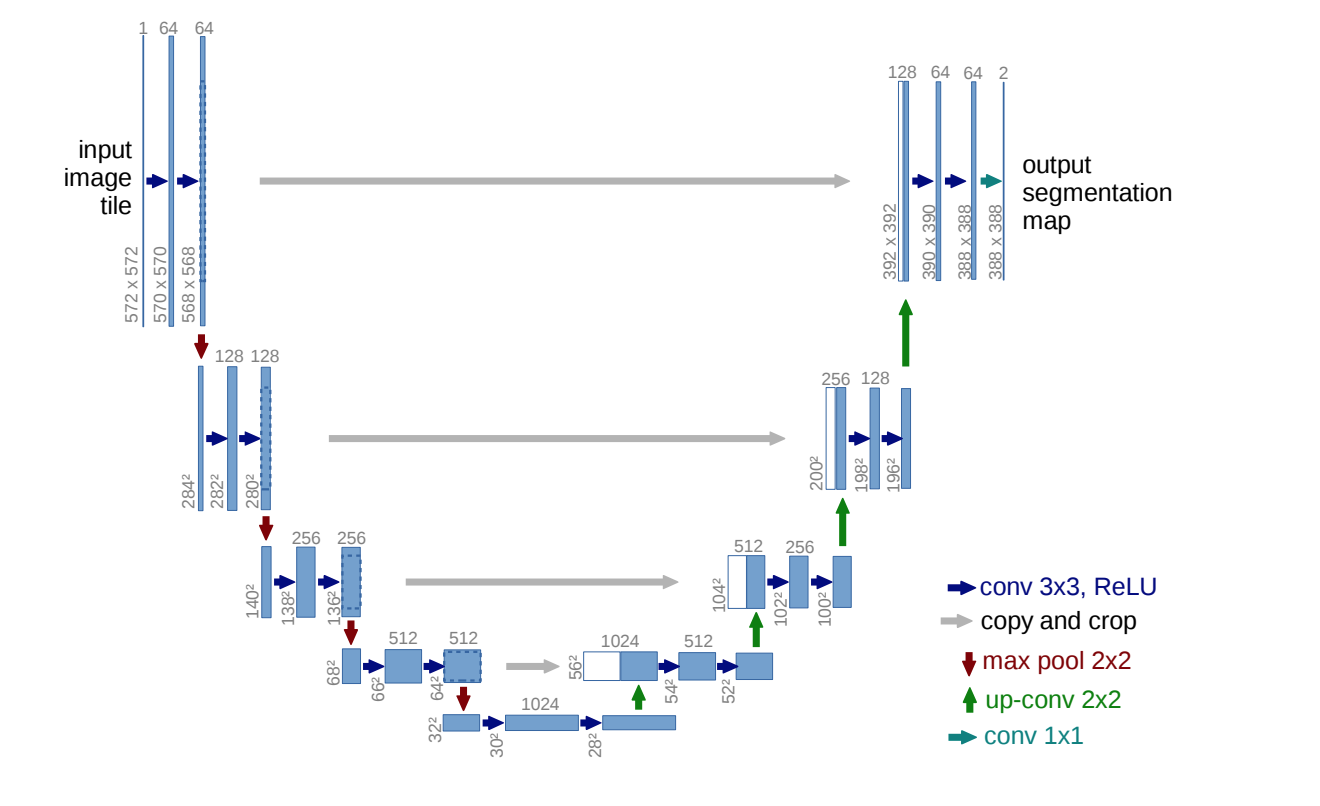
\includegraphics[width=10cm]{/home/thesis/images/UNet_Ronneberger.png}
    \caption{U-Net architecture, as illustrated in \cite{Ronneberger2015}. 
    Each blue box represents a multi-channel feature-map. 
    The number of channels is indicated above the box, the $x \times y$ dimensions are indicated at the bottom left.
    The gray arrows indicate the feature maps in the contracting path are copied and concatenated to the feature maps of the expanding path.}
    \label{fig:unet}
\end{SCfigure}

\todo[inline]{General introduction of U-Net and other medical approaches}

\subsection{Segmentation of the human spine}

\todo[inline]{other authors, approaches --> priors used, metrics used}

\section{Weakly supervised segmentation}

\subsection{General approaches}

\todo[inline]{How is this problem generally solved: PCAMS, WISE, ...}

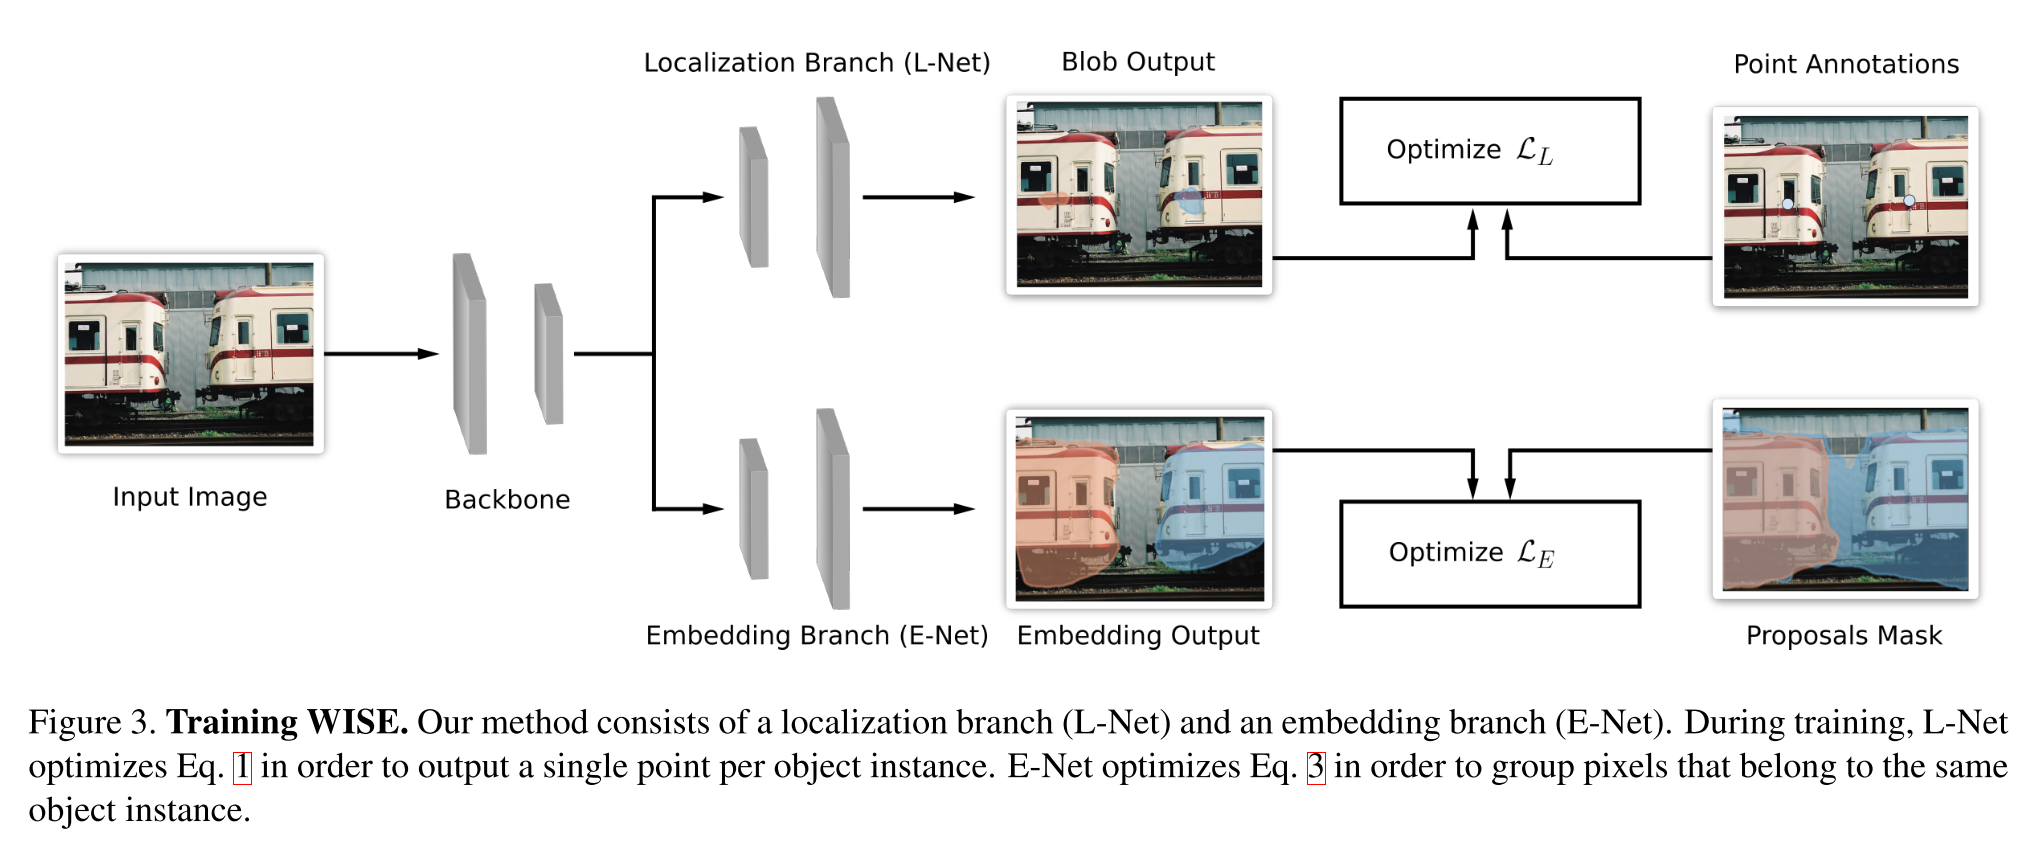
\includegraphics[width=10cm]{/home/thesis/images/Laradji_architecture.png}
\captionof{figure}{Architecture of the U-net based segmentation}
\label{fig:laradji}

\subsection{Weakly supervised segmentation for Medical applications}

Laradji COVID 19


\newgeometry{total={210mm,297mm},left=30mm,right=30mm,bindingoffset=5mm, top=25mm,bottom=25mm} 
\begin{partwithabstract}{Modelling \& Analysis}
    This part of the document details the used datasets and the modelling and evaluation methodology.
\end{partwithabstract}
\restoregeometry

\chapter{Datasets}

This thesis is based on 5 different already existing datasets.
This chapter discusses these datasets based on different criteria:

\begin{description}
    \item[source:] reference of the owner of the dataset and brief description of the original purpose of the dataset. Importantly, this part also discusses the source of the annotation.
    \item[Patient sample:] statistics of the patients of whom medical images were collected such as age, gender and possible spine pathologies.
    \item[Technical information:] discusses the imaging technology, the image resolution and the spatial dimensions of the image. 
\end{description}

\section{Global overview of the different dataset}

\todo[inline]{Overview of the datasets gathered. MRI / CT, number of images, type of annotation + WHO performed the annotation? Was it a medical docter or one of the researchers.}



bla

\begin{SCtable}[\sidecaptionrelwidth][h]
 
    \begin{tabular}{ l l l l l} 
     \hline
     \hline
     Name & reference & imaging & Quantity & Annotation \\
          &           & technology & [images] & \\
     \hline 
    UWSpine & \cite{Glocker}  & \acrshort{ct} & 125 & point  \\ 
    xVertSeg & \cite{Ibragimov2014, Korez2015} & \acrshort{ct} & 15 & full \\
    UniSiegen  & \cite{Zukic2014} & \acrshort{mri} & 17 & full \\
    PLoS & \cite{Chu2015} & \acrshort{mri} & 23 & semantic \\
    MyoSegmenTUM & \cite{Burian2019} & \acrshort{mri} &  54 & full \\
     \hline
     \hline
    \end{tabular}
    \caption{List of dataset references. For more details on the data quantity, please consult chapter \ref{seg:datasetcomparison}. 
    Notably the fact that some images were taken from the same patient is important. This means the dataset is grouped. 
    The agreement with prof. T. Vrtovec regarding the xVertSeg dataset can be found in appendix \ref{seg:datasetagreement}.}

\end{SCtable}

\begin{SCtable}[\sidecaptionrelwidth][h]
 
    \begin{tabular}{ l l l l} 
     \hline
     \hline
     Name & X & Y & Z \\
     \hline 
    UWSpine & Left-right & Anteroposterior & Craniocaudal \\
    xVertSeg & Left-right & Anteroposterior & Craniocaudal \\
    UniSiegen  &  Anteroposterior & Craniocaudal & Left-right \\
    PLoS & Left-right & Anteroposterior & Craniocaudal$^\dagger$ \\
    MyoSegmenTUM &  Anteroposterior & Craniocaudal & Left-right \\
     \hline
     \hline
    \end{tabular}
    \caption{List of dataset references. For more details on the data quantity, please consult chapter \ref{seg:datasetcomparison}. 
    Notably the fact that some images were taken from the same patient is important. This means the dataset is grouped. 
    The agreement with prof. T. Vrtovec regarding the xVertSeg dataset can be found in appendix \ref{seg:datasetagreement}.
    $^\dagger$ The Craniocaudal axis in the PLoS dataset is inverted.}

\end{SCtable}

\section{Comparison of the different datasets\label{seg:datasetcomparison}}


\subsection{xVertSeg\label{sec:xVertSeg}}



The xVertSeg \cite{Ibragimov2012, xxx} was kindly made available by prof. T. Vrtovec (University of Ljubljana, Faculty of Electrical Engineering, Slovenia), see appendix \ref{seg:datasetagreement} for the agreement.
This dataset contains 25 \acrfull{ct} scans of the lumbar spine, of which 15 \acrshort{ct} scans are fully labeled.
Given the provided data, I can assume these 15 scans were collected from 15 different patients.

For each of these 15 scans, full instance segmenation masks for all 5 lumbar vertebrae are provided. The delineation was performed by a skilled professional.

Additionally, for each vertebra a fracture class and fracture grade is provided. 
Apart from vertebrae classified as \textit{normal}, the dataset contains \textit{mild}, \textit{moderate} and \textit{severe} cases of vertebrae fracture types \textit{wedge}, \textit{crush} and \textit{biconcavity}.
\marginpar{
        % This file was created by tikzplotlib v0.9.8.
\begin{tikzpicture}

\definecolor{color0}{rgb}{0.917647058823529,0.917647058823529,0.949019607843137}
\definecolor{color1}{rgb}{0.298039215686275,0.447058823529412,0.690196078431373}
\definecolor{color2}{rgb}{0.768627450980392,0.305882352941176,0.32156862745098}

\begin{axis}[
axis background/.style={fill=color0},
axis line style={white},
height=5cm,
tick align=outside,
tick pos=left,
width=5cm,
x grid style={white},
xlabel={Gender},
xmajorgrids,
xmin=0.5, xmax=2.5,
xtick style={color=white!15!black},
xtick={1,2},
xticklabels={F (8),M (7)},
y grid style={white},
ylabel={Patient age [y]},
ymajorgrids,
ymin=0, ymax=100,
ytick style={color=white!15!black}
]
\addplot [color1, opacity=1]
table {%
0.925 66
1.075 66
1.075 79.25
0.925 79.25
0.925 66
};
\addplot [color1, opacity=1]
table {%
1 66
1 60
};
\addplot [color1, opacity=1]
table {%
1 79.25
1 90
};
\addplot [black, opacity=1]
table {%
0.9625 60
1.0375 60
};
\addplot [black, opacity=1]
table {%
0.9625 90
1.0375 90
};
\addplot [black, mark=o, mark size=3, mark options={solid,fill opacity=0}, only marks]
table {%
1 40
};
\addplot [color1, opacity=1]
table {%
1.925 73.5
2.075 73.5
2.075 78.5
1.925 78.5
1.925 73.5
};
\addplot [color1, opacity=1]
table {%
2 73.5
2 73
};
\addplot [color1, opacity=1]
table {%
2 78.5
2 82
};
\addplot [black, opacity=1]
table {%
1.9625 73
2.0375 73
};
\addplot [black, opacity=1]
table {%
1.9625 82
2.0375 82
};
\addplot [black, mark=o, mark size=3, mark options={solid,fill opacity=0}, only marks]
table {%
2 56
};
\addplot [color2, opacity=1]
table {%
0.925 72.5
1.075 72.5
};
\addplot [color2, opacity=1]
table {%
1.925 77
2.075 77
};
\end{axis}

\end{tikzpicture}

        \captionof{figure}{xVertSeg patients age distribution}
        \label{fig:xVertSeg_Age}
    }

\subsubsection{Original Objective of the Dataset}

The objective of the \textit{xVertSeg challenge}\footnote{see \url{http://lit.fe.uni-lj.si/xVertSeg/database.php}} (2015) was organized by the University of Ljubljana.
Based on the 15 provided scans with corresponding masks, the participans were required to construct a model to make predictions on the test set of 10 unlabelled scans.

The challenge consisted of two tasks:
\begin{enumerate}
    \item Segmentation of the lumbar vertebrae. For each scan in the test set, the segmentation masks of the lumbar vertebrae were requested.
    \item Fracture classification on the segmented vertebrae, consisting of morphological grade and fracture classification.
\end{enumerate}

\subsubsection{Patient statistics}

The patients in the xVertSeg dataset train set consist of 8 females and 7 males.
The age of these patients is slightly higher than for the other datasets.
The average patient in this dataset is 71 years old.
A box plot of the age distribution between genders is shown in figure \ref{fig:xVertSeg_Age}. 

\begin{SCtable}[\sidecaptionrelwidth][h]
    \centering
        \begin{tabular}{lrrrrrr}
\toprule
{} &  L1 &  L2 &  L3 &  L4 &  L5 &  Total \\
\midrule
biconcave &   6 &   7 &   8 &   4 &   2 &     27 \\
normal    &   5 &   6 &   4 &   4 &   7 &     26 \\
wedge     &   3 &   2 &   2 &   3 &   2 &     12 \\
crush     &   1 &   0 &   1 &   4 &   4 &     10 \\
\bottomrule
\end{tabular}

        \caption{Every patient in the xVertSeg dataset suffers from at least one spine pathology.
        Most of these pathologies are identified as \textit{mild}.
        This table counts the spine pathologies and normal vertebrae observed over all 15 patients in the xVertSeg dataset.}   
\end{SCtable}

\subsubsection{Technical information}

The xVertSeg dataset contains 15 \acrshort{ct} annotated scans. 
This dataset is very interesting due to the high quality and high resolution of the images.
On figure \ref{fig:xVertSeg_image002}, two slices of the same patient (002) are represented.
The slices show the complete, uncropped sections of the torso and abdominal region of the patient. 
There is no \acrshort{roi} cropping.

\begin{SCfigure}[][htb]
    \centering
    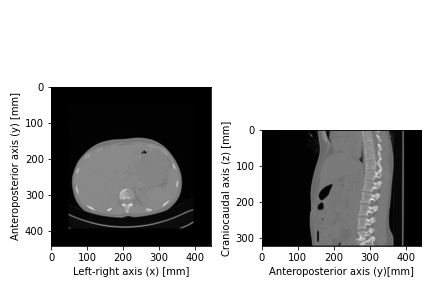
\includegraphics[width=.95\textwidth]{automated_graphs/xVertSeg_image002.png}
    \caption{xVertSeg scan \textit{image002}. \label{fig:xVertSeg_image002}}
\end{SCfigure}

The distribution of the scan dimensions is shown in figure \ref{fig:AllDataset_dims}. This also illustrates the \textit{xVertSeg} dataset consists of large, high resolution images.
Mind that during pre-processing the scans are resampled on a $1mm \times 1mm \times 1mm$ grid.


\subsection{UniSiegen dataset\label{sec:DataUSiegen}}

This dataset is made available in 2014 by the University of Siegen, Germany.
Dr D. Zukic \cite{Zukic2014} constructed it as part of his PhD project.

\marginpar{
        % This file was created by tikzplotlib v0.9.8.
\begin{tikzpicture}

\definecolor{color0}{rgb}{0.917647058823529,0.917647058823529,0.949019607843137}
\definecolor{color1}{rgb}{0.298039215686275,0.447058823529412,0.690196078431373}
\definecolor{color2}{rgb}{0.768627450980392,0.305882352941176,0.32156862745098}

\begin{axis}[
axis background/.style={fill=color0},
axis line style={white},
height=5cm,
tick align=outside,
tick pos=left,
width=5cm,
x grid style={white},
xlabel={Gender},
xmajorgrids,
xmin=0.5, xmax=2.5,
xtick style={color=white!15!black},
xtick={1,2},
xticklabels={F(11),M(6)},
y grid style={white},
ylabel={Patient age [y]},
ymajorgrids,
ymin=0, ymax=100,
ytick style={color=white!15!black}
]
\addplot [color1, opacity=1]
table {%
0.925 21.5
1.075 21.5
1.075 38.5
0.925 38.5
0.925 21.5
};
\addplot [color1, opacity=1]
table {%
1 21.5
1 21
};
\addplot [color1, opacity=1]
table {%
1 38.5
1 55
};
\addplot [black, opacity=1]
table {%
0.9625 21
1.0375 21
};
\addplot [black, opacity=1]
table {%
0.9625 55
1.0375 55
};
\addplot [black, mark=o, mark size=3, mark options={solid,fill opacity=0}, only marks]
table {%
1 74
1 69
};
\addplot [color1, opacity=1]
table {%
1.925 33
2.075 33
2.075 69.5
1.925 69.5
1.925 33
};
\addplot [color1, opacity=1]
table {%
2 33
2 27
};
\addplot [color1, opacity=1]
table {%
2 69.5
2 72
};
\addplot [black, opacity=1]
table {%
1.9625 27
2.0375 27
};
\addplot [black, opacity=1]
table {%
1.9625 72
2.0375 72
};
\addplot [color2, opacity=1]
table {%
0.925 22
1.075 22
};
\addplot [color2, opacity=1]
table {%
1.925 58
2.075 58
};
\end{axis}

\end{tikzpicture}

        \captionof{figure}{USiegen patients age distribution}
        \label{fig:USiegen_Age}
    }

This dataset contains 26 \acrshort{mri} scans of 17 different patients\footnote{This is not clearly stated, but can be inferred from the metadata.}. 
The fact that scans of the same patient are correlated will be taken into account in the train, validation and test split.
For more details on this split, see section \ref{sec:trainValTestSplit} on page \pageref{sec:trainValTestSplit}.

\subsubsection{Original Objective of the Dataset}

This dataset was collected from several hospitals (Sarajevo, Marburg, Brisbane, Schwabach, Bad Wildungen \& Prague). The MRI scanner settings were varied between the scans (T1, T2, TIRM).
The PhD project objective was to build a segmentation model to automate the segmentation of the lumbar vertebrae in the \acrshort{mri} scans to facilitate the diagnosis of several spine pathologies 
such as scoliosis, spondylolisthesis \footnote{Spondylolisthesis is the displacement of one spinal vertebra compared to another.} and vertebral fractures.
The final model developed by dr. D. Zukic consisted of a Viola-Jones detector for detection and vertebral body size approximation.
The average Dice score compared to the manual reference was reported to be 79.3\%.

\subsubsection{Patient statistics}

In \cite{Zukic2014}, it is not entirely made clear which scans are taken from the same patient.
It is made clear, however that the 26 scans were not obtained from 26 patients.
The information was inferred from the naming of the scans and the provided gender en age information\footnote{
    Wrongfully assuming two scans come from the same patient does not cause data leakage.
}.

Figure \ref{fig:USiegen_Age} illustrates that the USiegen dataset contains almost double the number of female patients compared to male patients.
These patients are relatively young compared to the patients in the \textit{xVertSeg} dataset.

Only three of the patients in this dataset were categorized as having no spinal pathologies.

\subsubsection{Technical information}

Several \acrlong{mri} techniques were used to obtain the dataset: T1, T2 \& TIRM.
I do not take into account this factor in the model development or the dataset split.

The volumes in the USiegen dataset are strongly cropped. 
Both in the anteroposterior and the craniocaudal direction, the volumes are on average 370 mm.
In the left-right direction, however, the volumes have been cropped severely. The volumes are, on average, only 68 mm wide.
The images have been cropped to only include the \acrshort{roi}.
Along this left-right dimension, the voxel spacing is large. 

\begin{SCfigure}[][htb]
    \centering
    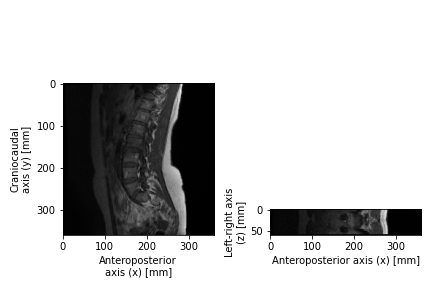
\includegraphics[width=.95\textwidth]{automated_graphs/USiegen_Aka3.png}
    \caption{USiegen dataset scan \textit{Aka3}. \label{fig:USiegen_Aka3}. It is immediately clear the USiegen volumes are cropped differently than the xVertSeg volumes.
    In the craniocaudal direction, both sacrum and coccyx are visible. Along the left-righ axis, the volumes have been cropped severely.}
\end{SCfigure}

The original scans in the \textit{USiegen} dataset were cropped in the \textit{left-right} direction. 
Although the scan resolution is relatively high in the Sagittal planes, the slice spacing along the left-right axis is coarser (see figure \ref{fig:AllDataset_dims}).  
\subsection{PLoS Dataset}

The \textit{PLoS} dataset was compiled for \cite{Chu2015} in 2015 by dr. C. Chu, University of Bern, Bern, Switzerland and made publically available \footnote{See : \url{ http://doi.org/10.5281/zenodo.22304 }} .
It consists of 23 T2-weighted spine \acrshort{mri} scans. 
Contrary to other datasets, the segmenation labels in this dataset do not provide information to destinguish the individual vertebrae from each other.

\subsubsection{Original Objective of the Dataset}

In \cite{Chu2015} the development of a random forest regression approach for spine vertebrae segmenation and classificiation is described.
The results of several random forest regressors and classifiers is unified with a voting mechanism.
This approach obtains a mean Dice metric score of 88.7\%.

\subsubsection{Patient statistics}

Due to the anomimization process, the \textit{PLoS} dataset does not contain patient information.
This means that it is not possible to produce any statistics regarding patient age or gender.

\subsubsection{Technical information}

As is indicated in figure \ref{fig:AllDataset_dims}, and in figure \ref{fig:PLoS_img02}, the PLoS image volumes are cropped in the left-right direction.
The volumes are consistently $381mm \times 381 mm \times 78 mm$, where the shortest dimension is in the left-right direction.

\begin{SCfigure}[][htb]
    \centering
    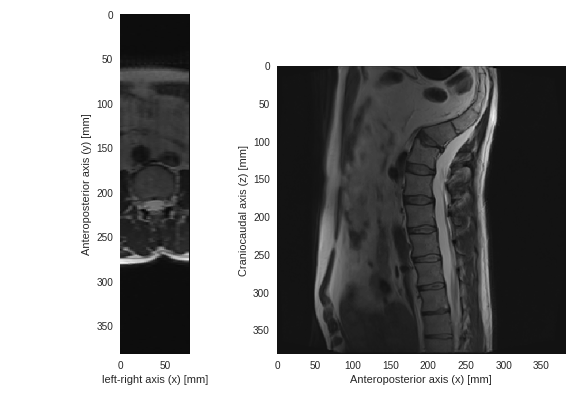
\includegraphics[width=.95\textwidth]{automated_graphs/PLoS_img02.png}
    \caption{
        PLoS dataset scan \textit{img02}. \label{fig:PLoS_img02}. The craniocaudal direction is cropped in a way comparable to the volumes in the USiegen dataset, but, the direction of this axis is inverted.
        The left-right axis is cropped similar to the USiegen data volumes.
    }
\end{SCfigure}
\subsection{MyoSegmenTUM datset}

This dataset is made available by S. Schläger from the Technische Universität München via the \acrfull{osf} \footnote{see \url{ https://osf.io/3j54b/?view_only=f5089274d4a449cda2fef1d2df0ecc56 }}.
It was constructed for the MyoSegmenTUM project \cite{Burian2019}.
It consists of 54 collections of \acrshort{mri} scans of the spine.
In this work, only the T2 weighted \acrlong{mri} scans are used.
The dataset also contains volumes with enhanced fat tissue response. Since the objective of this work is related to bone tissue rather than fat tissue, these volumes were not used.
Neither was the segmentation masks for the different dorsal muscles, which are also present in this dataset.

\subsubsection{Original Objective of the Dataset}

The MyoSegmenTUM Spine dataset is compiled as a reference dataset for developing segmentation algorithms of the lumbar spine vertebral bodies and muscle groups.
Information about this project can be found in \cite{Burian2019}.

\subsubsection{Patient statistics}

In figure \ref{fig:OSF_ageboxplot}, the age distribution of the patients in the MyoSegmenTUM dataset is shown.
There are more women (39) included in this dataset than men (15).
The male patients in this dataset are, on average, clearly younger than the female patients.

\marginpar{
        % This file was created by tikzplotlib v0.9.8.
\begin{tikzpicture}

\definecolor{color0}{rgb}{0.917647058823529,0.917647058823529,0.949019607843137}
\definecolor{color1}{rgb}{0.298039215686275,0.447058823529412,0.690196078431373}
\definecolor{color2}{rgb}{0.768627450980392,0.305882352941176,0.32156862745098}

\begin{axis}[
axis background/.style={fill=color0},
axis line style={white},
height=5cm,
tick align=outside,
tick pos=left,
width=5cm,
x grid style={white},
xlabel={Gender},
xmajorgrids,
xmin=0.5, xmax=2.5,
xtick style={color=white!15!black},
xtick={1,2},
xticklabels={F(39),M(15)},
y grid style={white},
ylabel={Patient age (y)},
ymajorgrids,
ymin=18.1666324435318, ymax=80.5007186858316,
ytick style={color=white!15!black}
]
\addplot [color1, opacity=1]
table {%
0.925 32.5
1.075 32.5
1.075 62.7652292950034
0.925 62.7652292950034
0.925 32.5
};
\addplot [color1, opacity=1]
table {%
1 32.5
1 21
};
\addplot [color1, opacity=1]
table {%
1 62.7652292950034
1 77.6673511293635
};
\addplot [black, opacity=1]
table {%
0.9625 21
1.0375 21
};
\addplot [black, opacity=1]
table {%
0.9625 77.6673511293635
1.0375 77.6673511293635
};
\addplot [color1, opacity=1]
table {%
1.925 27
2.075 27
2.075 33
1.925 33
1.925 27
};
\addplot [color1, opacity=1]
table {%
2 27
2 23
};
\addplot [color1, opacity=1]
table {%
2 33
2 41
};
\addplot [black, opacity=1]
table {%
1.9625 23
2.0375 23
};
\addplot [black, opacity=1]
table {%
1.9625 41
2.0375 41
};
\addplot [color2, opacity=1]
table {%
0.925 58.2888432580424
1.075 58.2888432580424
};
\addplot [color2, opacity=1]
table {%
1.925 31
2.075 31
};
\end{axis}

\end{tikzpicture}

        \captionof{figure}{Distribution of patient age in the dataset from the MyoSegmenTUM project.}
        \label{fig:OSF_ageboxplot}
    }


\subsubsection{Technical information}

As shown in figure \ref{fig:OSF_02}, coupes from the second volume of the MyoSegmenTUM dataset are shown.
As is also indicated in figure \ref{fig:AllDataset_dims}, the dimensions of the MyoSegmenTUM volumes is consistent $220 mm \times 220 mm \times 80 mm$, where the shortest dimension is the cropped left-right axis.
There are only three volumes that deviate slightly from this.

\begin{SCfigure}[][htb]
    \centering
    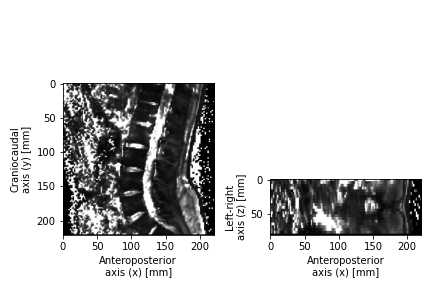
\includegraphics[width=.95\textwidth]{automated_graphs/OSF_02.png}
    \caption{MyoSegmenTUM dataset scan \textit{02}. 
    The volumes are cropped in the left-right direction. 
    \label{fig:OSF_02}}
\end{SCfigure}

\textbf{Remark:} For three volumes (nr 33, 53 and 54) for which the dimension of the image volume and the label mask do not correspond. 
It is not clear how these masks should be used. 
These volumes were discarded, bringing the final number of volumes used from the MyoSegmenTUM dataset to 51.
\subsection{UWSpine dataset}
 
This dataset is made available by the Department of Radiology of the University of Washington\footnote{Creative Commons Attribution-NonCommercial-NoDerivatives 4.0 International License, dataset available at \url{
      https://biomedia.doc.ic.ac.uk/data/spine/  
    }}.
It has been constructed by dr. Glocker and team \cite{Glocker2012,Glocker2013} (Microsoft research) in 2012.
For each scan, manual annotations of vertebrae centroids are provided.
This dataset contains 242 \acrshort{ct} scans of 150 different patients.
This dataset does not contain full mask labels, only centroid point annotations.
To investigate the relative performance of a weakly supervised model compared to the performance of a fully supervised model, both will be trained on the same dataset\footnote{The modelling concept is further discussed in chapter \ref{sec:model_concept}.}.
Furthermore, the evaluation of the models is based on the full annotations.
Thus, the UWSpine dataset will not be used for model training.
It will only be used for visual evaluation of the model on a completely new dataset\footnote{The UWSpine dataset is \textit{completely} new in the sense that no samples from this dataset (this \textit{population}, so to speak) are present in the train or validation set.
For the \textit{normal} test set, other samples from the same datasets where present in the train and validation sets.}.


\subsubsection{Original Objective of the Dataset}

In \cite{Glocker2012,Glocker2013} the development of a model based on regression forests and a \acrfull{hmm} for vertebra localisation without needing strong assumptions on what part of the spine is visible.

\subsubsection{Patient statistics}


Figure \ref{fig:UW_ageboxplot} illustrated that the patients in the \textit{UWSpine} dataset are relatively varied in age.
Of most patients in the dataset, multiple scan images are available.
The highest number of scans taken from a single patient is 5.

\subsubsection{Technical information}

Only point annotations are available for the \textit{UWSpine} dataset. 
This means this dataset can only be used for weakly supervised model training.

The scans in the \textit{UWSpine} dataset are strongly cropped around the spine, both in the left-right direction and the anteroposterior direction.

\begin{SCfigure}[][htb]
    \centering
    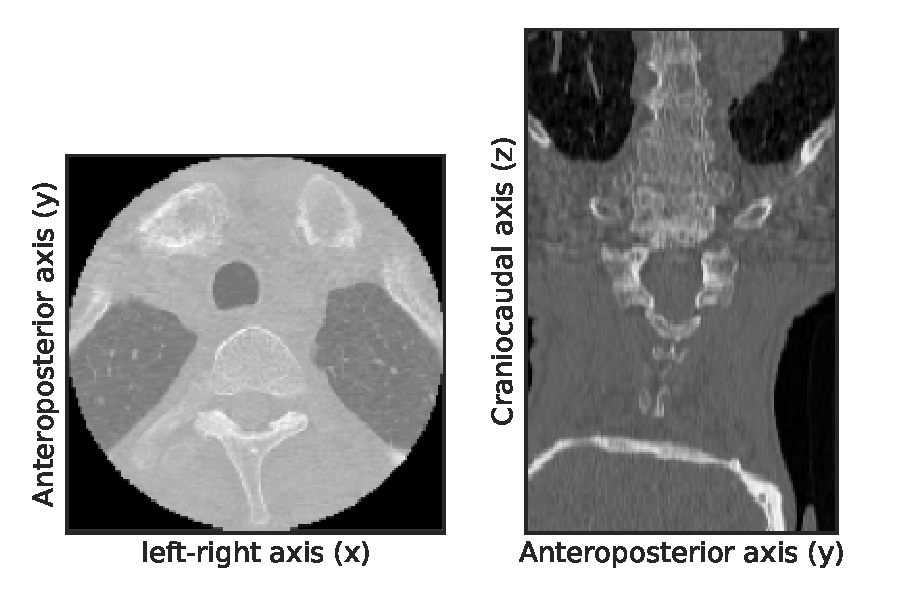
\includegraphics[width=.95\textwidth]{automated_graphs/UW_4564688.pdf}
    \caption{University of Washington dataset, scan \textit{4564688}. \label{fig:UW_4564688}}
\end{SCfigure}

\marginpar{
        % This file was created by tikzplotlib v0.9.8.
\begin{tikzpicture}

\definecolor{color0}{rgb}{0.917647058823529,0.917647058823529,0.949019607843137}
\definecolor{color1}{rgb}{0.298039215686275,0.447058823529412,0.690196078431373}
\definecolor{color2}{rgb}{0.768627450980392,0.305882352941176,0.32156862745098}

\begin{axis}[
axis background/.style={fill=color0},
axis line style={white},
tick align=outside,
tick pos=left,
x grid style={white},
xlabel={Gender},
xmajorgrids,
xmin=0.5, xmax=2.5,
xtick style={color=white!15!black},
xtick={1,2},
xticklabels={Female (54 patients),Male (71 patients)},
y grid style={white},
ylabel={Patient age (y)},
ymajorgrids,
ymin=11.05, ymax=97.95,
ytick style={color=white!15!black}
]
\addplot [color1, opacity=1]
table {%
0.925 42.75
1.075 42.75
1.075 64.75
0.925 64.75
0.925 42.75
};
\addplot [color1, opacity=1]
table {%
1 42.75
1 15
};
\addplot [color1, opacity=1]
table {%
1 64.75
1 94
};
\addplot [black, opacity=1]
table {%
0.9625 15
1.0375 15
};
\addplot [black, opacity=1]
table {%
0.9625 94
1.0375 94
};
\addplot [color1, opacity=1]
table {%
1.925 41.5
2.075 41.5
2.075 65.5
1.925 65.5
1.925 41.5
};
\addplot [color1, opacity=1]
table {%
2 41.5
2 15
};
\addplot [color1, opacity=1]
table {%
2 65.5
2 90
};
\addplot [black, opacity=1]
table {%
1.9625 15
2.0375 15
};
\addplot [black, opacity=1]
table {%
1.9625 90
2.0375 90
};
\addplot [color2, opacity=1]
table {%
0.925 54
1.075 54
};
\addplot [color2, opacity=1]
table {%
1.925 54
2.075 54
};
\end{axis}

\draw ({$(current bounding box.south west)!0.5!(current bounding box.south east)$}|-{$(current bounding box.south west)!0.98!(current bounding box.north west)$}) node[
  scale=0.6,
  anchor=north,
  text=white!15!black,
  rotate=0.0,
  align=center
]{OSF dataset
age distribution};
\end{tikzpicture}

        \captionof{figure}{Distribution of patient age in the dataset from Washington University.}
        \label{fig:UW_ageboxplot}
    }


\chapter{Proposed methods}

\section{Comparison between Fully supervised and Weakly supervised models}

\section{Fully supervised model}

\section{Weakly supervised model}

\chapter{Experiments}

\section{Experimental results of the fully supervised model}

\section{Experimental results of the weakly supervised model}

\section{Comparison between fully \& weakly supervised model}

\section{Final model proposal}

\section{Experimental results of the final model}

\chapter{Conclusion}

Comparison between results with weakly supervised model and fully supervised model.

\appendix

\newgeometry{total={210mm,297mm},left=30mm,right=30mm,bindingoffset=5mm, top=25mm,bottom=25mm}
\begin{partwithabstract}{Appendix}
  Apendices to the document:
  \begin{enumerate}
    \item Software environment used
    \item Agreement documents for use of two datasets.
  \end{enumerate}
\end{partwithabstract}
\restoregeometry
\chapter{Used software}

\todo[inline]{Software environments can be build with dockerfiles available in folder \textit{/dockerfiles/code/} of the git.}

\todo[inline]{Assure proper referencing of all libraries used}

\begin{SCtable}[\sidecaptionrelwidth][h]
 
  \begin{tabular}{ p{6cm} l l } 
   \hline
   \hline
   Library & version & reference  \\
   \hline 
   PyTorch & 1.7.1 &  \\ 
   SimpleITK &  &  \\ 
   \hline
   \hline
  \end{tabular}
  \caption{Python libraries used}

\end{SCtable}
\newgeometry{total={210mm,297mm},left=30mm,right=30mm,bindingoffset=5mm, top=25mm,bottom=25mm}
\chapter{Dataset agreements}

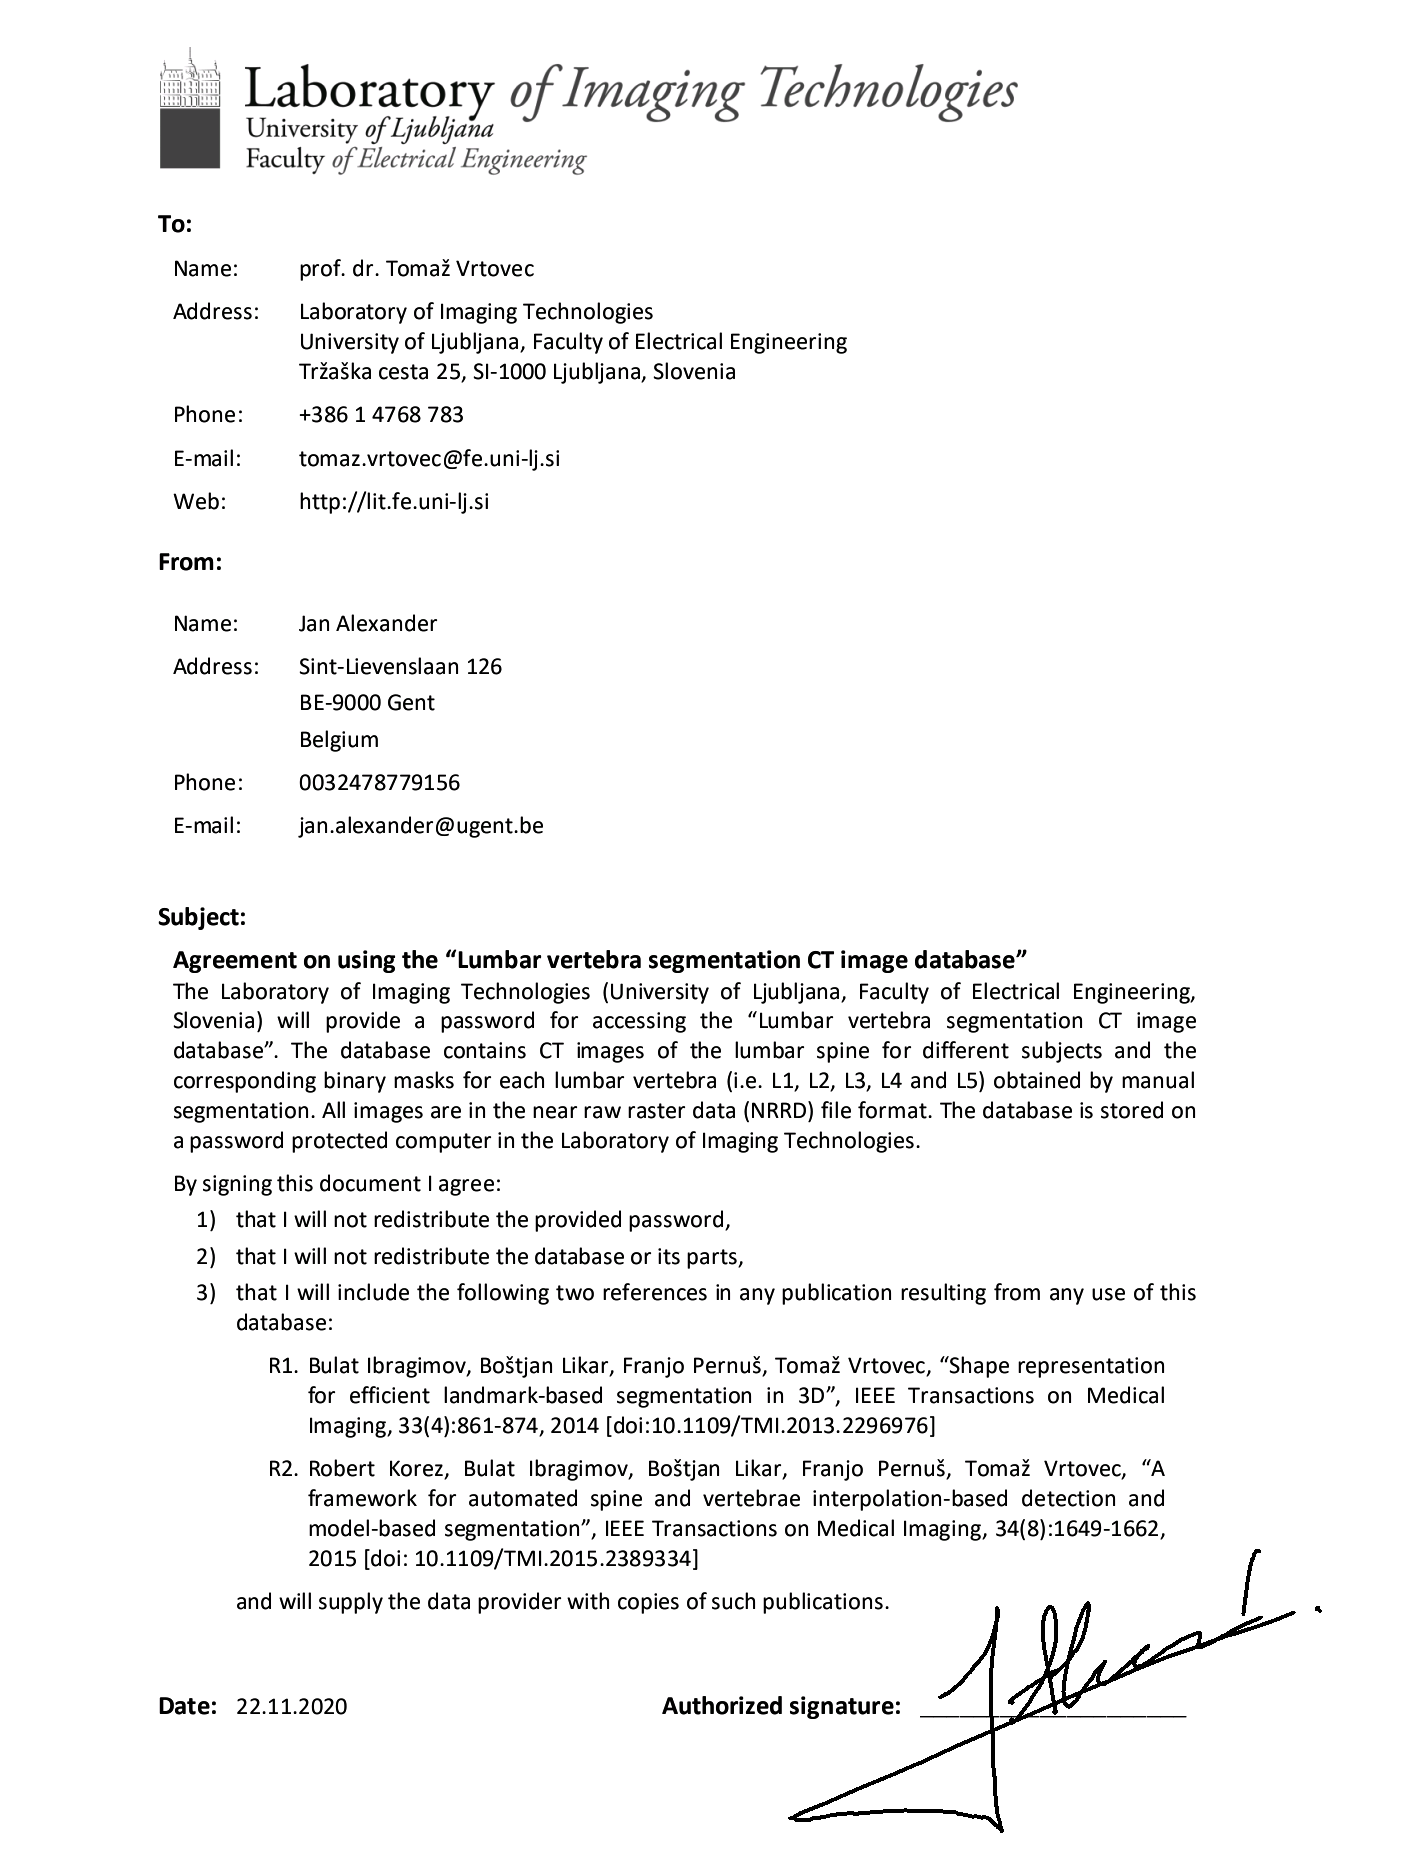
\includegraphics[width=17cm]{/home/thesis/images/AgreementxVertSeg.png}

\printbibliography

\end{document}

